\chapter{Componetele unei aplica\c tii Android}

Framework-ul Android ofer\u a o serie de componente pentru dezvoltarea de aplica\c tii consistente \c si interoperabile. \^In continuare vor fi prezentate componentele fundamentale oferite de platforma Android.\cite{3}
\begin{center}
\begin{figure}[!hp]
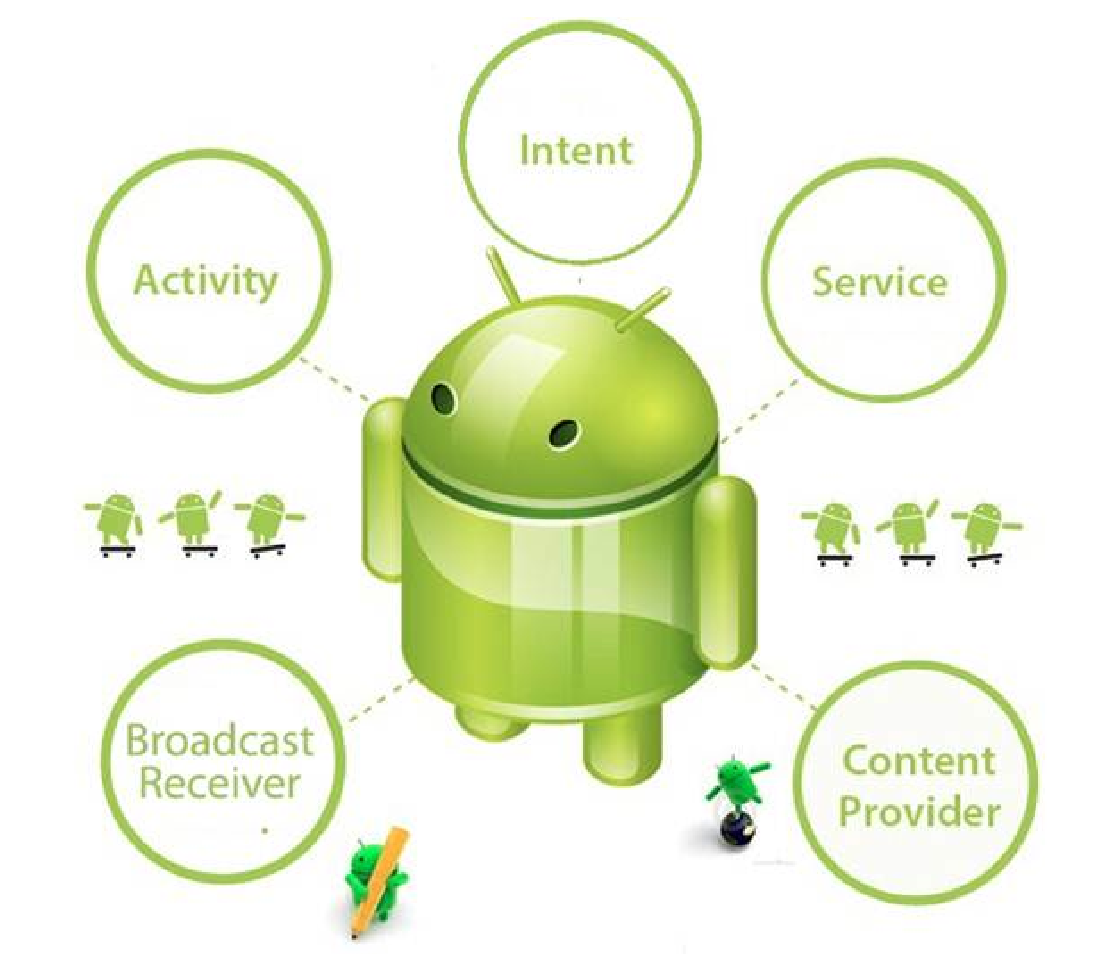
\includegraphics[width=0.65\textwidth]
{imagini/components-of-android.eps}
\end{figure}
\end{center}

\section{Activity}

,,Activity'' este numele dat pentru o aplica\c tie \^in care utilizatorul poate interac\c tiona cu o singur\u a fereastr\u a la un moment dat. A fost ales numele de ,,activitate'' pentru a sugera faptul c\u a aplica\c tia poate s\u a realizeze o singur\u a func\c tionalitate focusat\u a pe utilizator.\newline 
Pe platforma Android, acest aspect de limitare al domeniului fiecarui ecran aduce func\c tionalitea de interac\c tionare cu alte aplica\c tii. De exemplu, la utilizarea e-mail-ului pe un dispozitiv mobil, c\^and userul are posibilitatea de a selecta un contact din lista de contacte c\u aruia s\u a-i trimit\u a e-mail-ul.\newline 

Acest lucru face posibil\u a reutilizarea codului \c si men\c tinerea platformei in str\^ans\u a leg\u atura.\newline
Aproape toate aplica\c tiile necesit\u a comunicarea \c si/sau interac\c tionarea cu un client, \c si din acest motiv, activitatea se ocup\u a de crearea unei ferestre \c si de a\c sezarea componentelor interfetei utilizator.\cite{3}\newline 

\subsection{Crearea unei activit\u a\c ti}
Pentru a crea o nou\u a activitate se deriveaz\u a o clasa din android.app.Activity, dup\u a cum putem observa \^in exemplul 3.1.\cite{3}\newline 

\begin{exmp} Crearea unei activit\u a\c ti\newline 
import android.app.Activity;\newline 
public class MyActivity extends Activity \{\newline 
\}\end{exmp}

\subsection{Declararea unei activit\u a\c ti}
Derivarea unei clase de acvitate nu \^inseamn\u a \c si faptul c\u a acea activitate este automat utilizabil\u a. Pentru ca o activitate s\u a ia anumite roluri \^in aplicatie, platforma Android necesit\u a ni\c ste meta-informa\c tii despre noua activitate. Aceste informa\c tii sunt furnizate de c\u atre fisierul XML Android manifest, unde eticheta XML /<activity/> declar\u a noua activitate prin precizarea numelui de clas\u a, a titlului \c si a modului \^in care va fi expus\u a utilizatorului.\cite{1}\newpage

\subsection{Ciclul de via\c t\u a al unei activit\u a\c ti}\cite{1}

\begin{center}
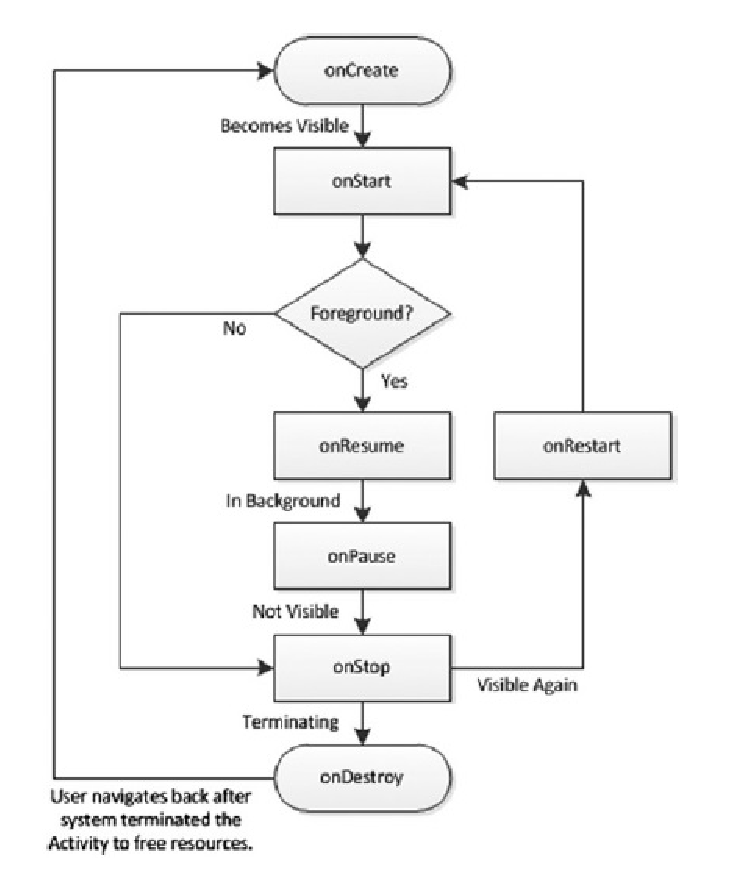
\includegraphics[width=0.6\textwidth]{imagini/activity.eps}
\end{center}

\section{Intent}
Dup\u a cum am men\c tionat \c si anterior, platforma Android este dezvoltat\u a pentru a fi extrem de modular\u a, promov\^ and colaborarea dintre aplica\c tiile prezente pe dispozitiv. Astfel, aplica\c tiile pot \^imbina activit\u a\c ti pentru a oferi o anumit\u a func\u tionalitate utilizatorului. Acest lucru este posibil printr-un binding runtime \^int\^arziat, cunoscut sub numele de android.content.Intent, pe care platforma Android \^il pune la dispozi\c tie.\newline 
Intent-ul de\c tine o structur\u a pasiv\u a de date care memoreaz\u a o descriere abstract\u a a ac\c tiunii ce urmeaz\u a a fi \^intreprins\u a. Principalele informa\c tii dintr-un intent sunt:\newline 

\begin{itemize}
  \item action, care reprezint\u a \^in general ac\c tiunea ce va fi \^intreprins\u a
  \item data, care reprezint\u a un obiect URI (uniform resource identifier) ce se refer\u a la datele care vor fi prelucrate
\end{itemize}
Cea mai important\u a utilizare a intentului este de a lansa activit\u a\c tile si serviciile.

\section{Service}
Pentru aplica\c tii cu durat\u a de rulare mai mare, durata de via\c t\u a a unei activit\u a\c ti s-ar putea s\u a nu fie indeajuns de lung\u a, de exemplu daca o aplica\c tie necesit\u a desc\u arcarea de pe Internet a unui videoclip, platforma va termina activitatea imediat dup\u a ce utilizatorul p\u araseste temporar aplica\c tia fără a verifica dac\u a opera\c tia s-a incheiat sau nu.\newline 
Framework-ul Android furnizeaz\u a o component\u a a aplica\c tiei, numit\u a android.app.Service, pentru a permite aplica\c tiilor s\u a execute opera\c tii cu durrata de rulare mai mare \^in planul secundar.\newline 
Serviciile pot fi utilizate \c si din aceeasi aplica\c tie dar \c si de alte aplica\c tii  de pe dispozitiv dac\u a serviciul este exportat.\cite{1}


\subsection{Crearea unui Service}
Crearea unui serviciu se face prin simpla derivare a unei noi clase din android.app.Service cum se vede \^in exemplul 3.2.\cite{2}\newline 
\begin{exmp} Crearea unui Service
import android.app.Service;\newline 
public class MyService extends Service \{ \newline 
\} \end{exmp}

\subsection{Declararea unui Service}
Crearea unui noi serviciu nu \^il face imediat utilizabil pe platforma Android. Aceasta are nevoie de meta-informa\c tii pentru a putea utiliza serviciul. Aceste meta-informa\c tii se g\u asesc \^, de asemnea \^in  fi\c sierul Android manifest fiind marcate cu tagul XML <service>.\newline 
Asemenea elementului <activity>, elementul <service> poate s\u a con\c tina elemente <intent-filter> \^in corpul s\u au pentru a specifica ce ac\c tiuni s\u a indeplineasc\u a.\cite{2}

\subsection{Ciclul de via\c t\u a al unui Service}
\begin{center}
\caption{\cite[1]}
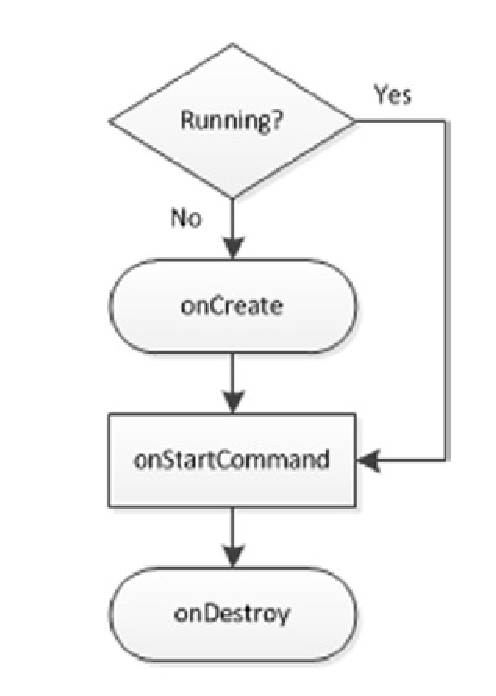
\includegraphics[width=0.3\textwidth]{imagini/service.eps}
\end{center}

\newpage
\section{Content Provider}
Dup\u a cum am men\c tionat anterior \^in sec\c tiunea ,,Service'', at\^ at activit\u a\c tile c\^ at \c si serviciile pot fi exportate astfel \^incat alte aplicatii care ruleaz\u a pe acela\c si dispozitiv mobil s\u a poat\u a interac\c tiona simultan cu acestea. Chiar dac\u a accesarea unor p\u ar\c ti ale altor aplica\c tii poate fi foarte util\u a, \^in anumite cazuri, este nevoie de simpla accesare a datelor, f\u ar\u a accesarea anterioar\u a a activit\u a\c tilor si a serviciului.\newline 
Platforma Android furnizeaza o component\u a aplica\c tiei, numit\u a content provider, care manageriaz\u a accesul la un set structurat de date. Este o interfa\c t\u a standard care conecteaz\u a datele unei aplica\c tii cu codul executabil al altei aplica\c tii.\cite{2}\newline 

\subsection{Crearea unui Content Provider}
Un nou content provider poate fi creat prin simpla derivare a unei noi clase din android.content.ContentProvider ca \^in exemplul 3.3.\newline 
\begin{exmp} Crearea unui Content Provider 
import android.content.ContentProvider;\newline 
public class MyContentProvider extends ContentProvider \{\newline 
\}\end{exmp}

Clasa abstract\u a ContentProvider cuprinde 6 metode abstracte care necesită implementare.\cite{2}

\begin{itemize}
  \item query - metodă apelat\u a pentru a interoga providerul pentru date 
  \item insert - metodă apelat\u a pentru a insera continut nou in provider
	\item update - metodă apelat\u a pentru a actualiza continutul unui provider cu un nou conținut
	\item delete-  metodă  apelat\u a pentru a sterge providerul
	\item getType -metodă apelat\u a pentru a prelua tipul MIME pentru conținutul ce va fi returnat pentru URI-ul dat
	\item onCreate - metodă apelat\u a de platform\u a c\^and se instan\c tiaz\u a providerul.(apelat\u a inainte de orice altă metod\u a)
\end{itemize}
\newpage
\section{Broadcast Messages}
Platforma Android furnizeaz\u a un sistem larg de mesagerie numit broadcast messages. Aceast\u a facilitate permite aplica\c tiilor \c si sistemului s\u a propage evenimente \c si schimb\u ari de stare pentru par\c tile interesate prin emiterea unui intent ca mesaj.\newline 
Un mesaj broadcast poate fi trimis prin metoda sendBroadcast. \newline 
Pentru receptarea unui mesaj broadcast, aplica\c tia trebuie s\u a deriveze o nou\u a clas\u a din android.content.BroadcastReceiver. \newline 

Simpla derivare a clasei nu este ins\u a suficientă pentru a recep\c tiona mesajele. Aplica\c tia trebuie s\u a informeze platforma Android dinamic prin cod sau prin \^inregistrarea \^in fisierul manifest cu privire la intenția de a recep\c tiona mesaje broadcast.\newline
Tagul XML <receiver> este utilizat pentru a \^inregistra un receptor broadcast \^in manifestul aplica\c tiei.\newline
Pentru \^inregistrarea dinamic\u a prin cod, exist\u a metoda registerReceiver.\cite{1}\newline
